% A simple fault tree
% Author: Zhang Long, Mail: zhangloong[at]gmail.com
%\def\pgfsysdriver{pgfsys-dvipdfm.def}
\documentclass{article}\usepackage[]{graphicx}\usepackage[]{xcolor}
% maxwidth is the original width if it is less than linewidth
% otherwise use linewidth (to make sure the graphics do not exceed the margin)
\makeatletter
\def\maxwidth{ %
  \ifdim\Gin@nat@width>\linewidth
    \linewidth
  \else
    \Gin@nat@width
  \fi
}
\makeatother

\definecolor{fgcolor}{rgb}{0.345, 0.345, 0.345}
\newcommand{\hlnum}[1]{\textcolor[rgb]{0.686,0.059,0.569}{#1}}%
\newcommand{\hlstr}[1]{\textcolor[rgb]{0.192,0.494,0.8}{#1}}%
\newcommand{\hlcom}[1]{\textcolor[rgb]{0.678,0.584,0.686}{\textit{#1}}}%
\newcommand{\hlopt}[1]{\textcolor[rgb]{0,0,0}{#1}}%
\newcommand{\hlstd}[1]{\textcolor[rgb]{0.345,0.345,0.345}{#1}}%
\newcommand{\hlkwa}[1]{\textcolor[rgb]{0.161,0.373,0.58}{\textbf{#1}}}%
\newcommand{\hlkwb}[1]{\textcolor[rgb]{0.69,0.353,0.396}{#1}}%
\newcommand{\hlkwc}[1]{\textcolor[rgb]{0.333,0.667,0.333}{#1}}%
\newcommand{\hlkwd}[1]{\textcolor[rgb]{0.737,0.353,0.396}{\textbf{#1}}}%
\let\hlipl\hlkwb

\usepackage{framed}
\makeatletter
\newenvironment{kframe}{%
 \def\at@end@of@kframe{}%
 \ifinner\ifhmode%
  \def\at@end@of@kframe{\end{minipage}}%
  \begin{minipage}{\columnwidth}%
 \fi\fi%
 \def\FrameCommand##1{\hskip\@totalleftmargin \hskip-\fboxsep
 \colorbox{shadecolor}{##1}\hskip-\fboxsep
     % There is no \\@totalrightmargin, so:
     \hskip-\linewidth \hskip-\@totalleftmargin \hskip\columnwidth}%
 \MakeFramed {\advance\hsize-\width
   \@totalleftmargin\z@ \linewidth\hsize
   \@setminipage}}%
 {\par\unskip\endMakeFramed%
 \at@end@of@kframe}
\makeatother

\definecolor{shadecolor}{rgb}{.97, .97, .97}
\definecolor{messagecolor}{rgb}{0, 0, 0}
\definecolor{warningcolor}{rgb}{1, 0, 1}
\definecolor{errorcolor}{rgb}{1, 0, 0}
\newenvironment{knitrout}{}{} % an empty environment to be redefined in TeX

\usepackage{alltt}
\usepackage{tikz}
\usetikzlibrary{shapes.gates.logic.US, trees, positioning, arrows}
\IfFileExists{upquote.sty}{\usepackage{upquote}}{}
\begin{document}
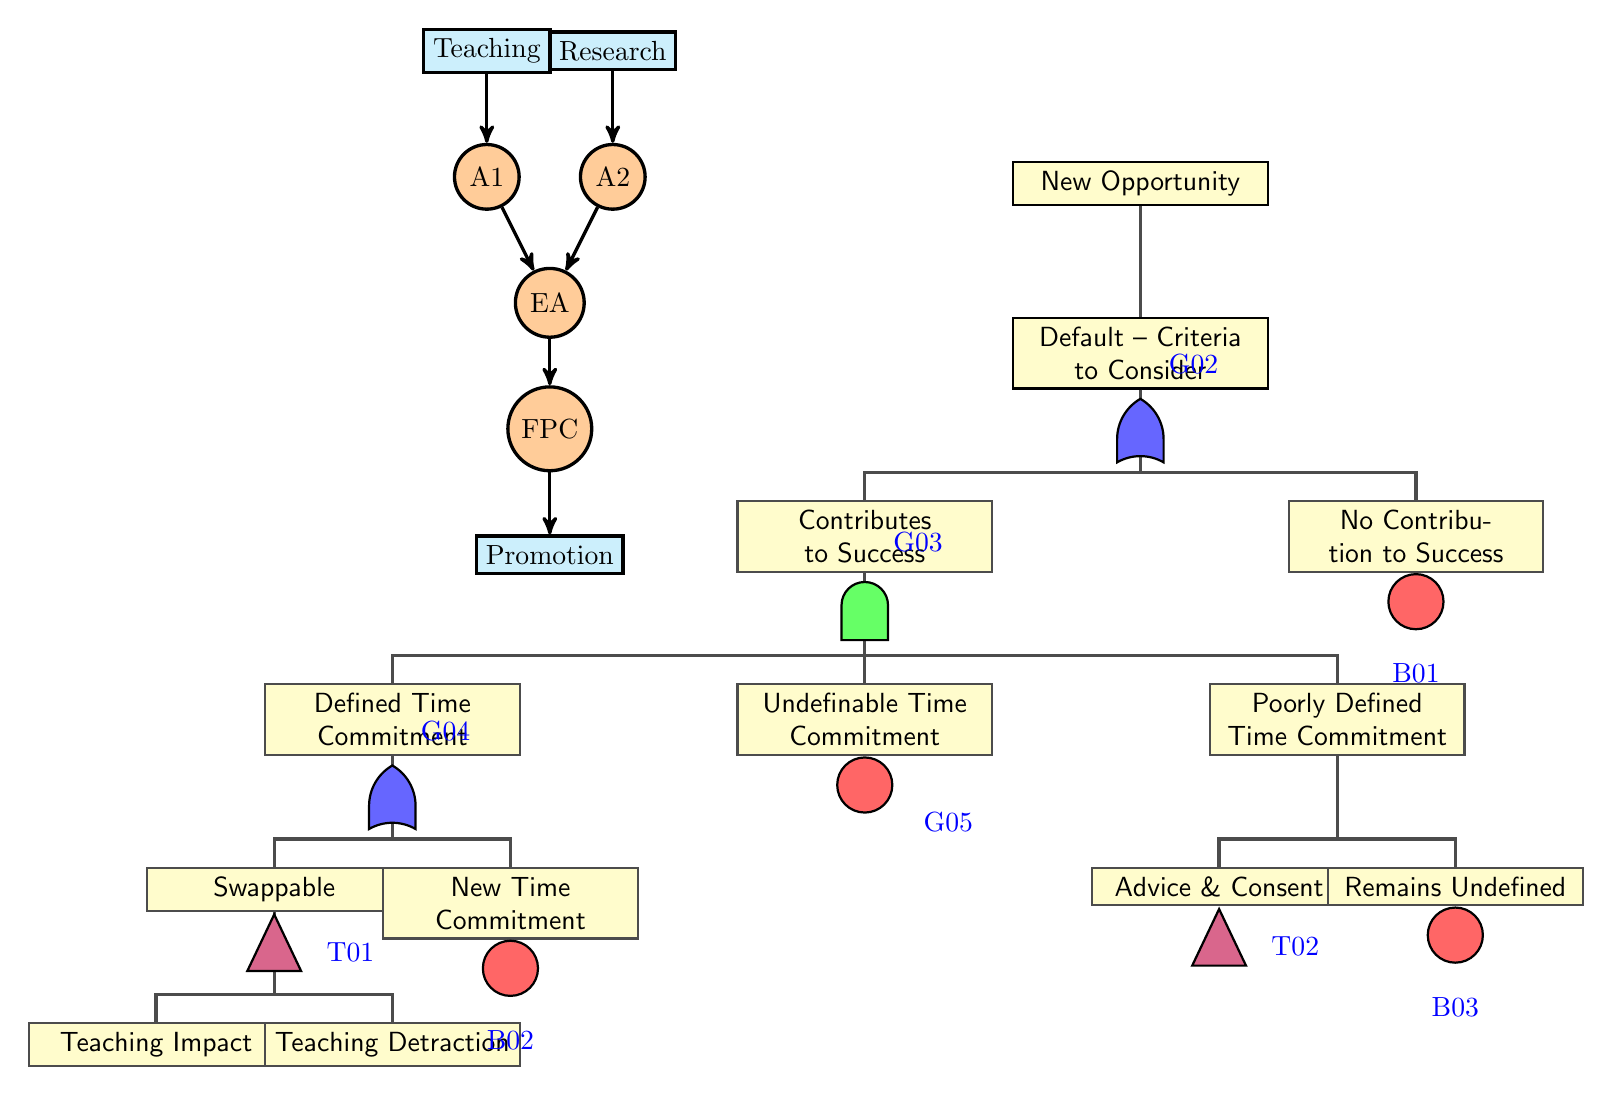
\begin{tikzpicture}[
% Gates and symbols style
    and/.style={and gate US,thick,draw,fill=green!60,rotate=90,
		anchor=east,xshift=-1mm},
    or/.style={or gate US,thick,draw,fill=blue!60,rotate=90,
		anchor=east,xshift=-1mm},
    no/.style={circle,thick,draw,fill=red!60,anchor=north,
		minimum width=0.7cm},
    may/.style={buffer gate US,thick,draw,fill=purple!60,rotate=90,
		anchor=east,minimum width=0.8cm},
% Label style
    label distance=3mm,
    every label/.style={blue},
% Event style
    event/.style={rectangle,thick,draw,fill=yellow!20,text width=3cm,
		text centered,font=\sffamily,anchor=north},
% Children and edges style
    edge from parent/.style={very thick,draw=black!70},
    edge from parent path={(\tikzparentnode.south) -- ++(0,-1.05cm)
			-| (\tikzchildnode.north)},
    level 1/.style={sibling distance=7cm,level distance=1.4cm,
			growth parent anchor=south,nodes=event},
    level 2/.style={sibling distance=7cm},
    level 3/.style={sibling distance=6cm},
    level 4/.style={sibling distance=3cm},
    level 5/.style={sibling distance=3cm}
%%  For compatability with PGF CVS add the absolute option:
%   absolute
    ]
%% Draw events and edges
    \node (g1) [event] {New Opportunity}
	     child{node (g2) {Default -- Criteria to Consider}   
	     	child {node (g3) {Contributes to Success}
	     	   child {node (g4) {Defined Time Commitment}
	     	      child {node (t1) {Swappable}
	     	        child {node (d1) {Teaching Impact}}
	     	        child {node (d2) {Teaching Detraction}}
	     	      }
	     	      child {node (b2) {New Time Commitment}}
			}
	     	   child {node (g5) {Undefinable Time Commitment}}
	     	   child {node (g6) {Poorly Defined Time Commitment}
	     	      child {node (t2) {Advice \& Consent}}
	     	      child {node (b3) {Remains Undefined}}
			}
		   }
	     	child {node (b1) {No Contribution to Success}}
		};
%% Place gates and other symbols
%% In the CVS version of PGF labels are placed differently than in PGF 2.0
%% To render them correctly replace '-20' with 'right' and add the 'absolute'
%% option to the tikzpicture environment. The absolute option makes the 
%% node labels ignore the rotation of the parent node. 
   \node [or]	at (g2.south)	[label=-20:G02]	{};
   \node [and]	at (g3.south)	[label=-20:G03]	{};
   \node [or]	at (g4.south)	[label=-20:G04]	{};
   \node [no]	at (g5.south)	[label=-20:G05]	{};
   \node [no]	at (b1.south)	[label=below:B01]	{};
   \node [no]	at (b2.south)	[label=below:B02]	{};
   \node [no]	at (b3.south)	[label=below:B03]	{};
   \node [may]	at (t1.south)	[label=below:T01]	{};
   \node [may]	at (t2.south)	[label=below:T02]	{};
%% Draw system flow diagram
   \begin{scope}[xshift=-7.5cm,yshift=-5cm,very thick,
		node distance=1.6cm,on grid,>=stealth',
		block/.style={rectangle,draw,fill=cyan!20},
		comp/.style={circle,draw,fill=orange!40}]
   \node [block] (re)					{Promotion};
   \node [comp]	 (cb)	[above=of re]			{FPC}  edge [->] (re);
   \node [comp]  (cc) [above=of cb]     {EA}   edge [->] (cb);
   \node [comp]	 (ca1)	[above=of cc,xshift=-0.8cm]	{A1} edge [->] (cc);
   \node [comp]	 (ca2)	[right=of ca1]			{A2} edge [->] (cc);
   \node [block] (s1)	[above=of ca1]		{Teaching} edge [->] (ca1);
   \node [block] (s2)	[right=of s1]		{Research} edge [->] (ca2);
   \end{scope}
\end{tikzpicture}
\end{document}
